\documentclass[oneside,11pt,letter]{article}

% General include (DO NOT MODIFY)
\usepackage{amsmath,graphicx,cite,latexsym,color, amssymb,ifthen,verbatim}

\usepackage{listings}
\definecolor{mygreen}{rgb}{0,0.6,0}
\definecolor{mygray}{rgb}{0.5,0.5,0.5}
\definecolor{mymauve}{rgb}{0.58,0,0.82}

\lstset{ %
  backgroundcolor=\color{white},   % choose the background color
  basicstyle=\footnotesize,        % size of fonts used for the code
  breaklines=true,                 % automatic line breaking only at whitespace
  captionpos=b,                    % sets the caption-position to bottom
  commentstyle=\color{mygreen},    % comment style
  escapeinside={\%*}{*)},          % if you want to add LaTeX within your code
  keywordstyle=\color{blue},       % keyword style
  stringstyle=\color{mymauve},     % string literal style
}
\lstset{basicstyle=\small\ttfamily,breaklines=true}

%--------------- Various Style Declarations ----------------------------
\textheight 9in
\topmargin 0in
\headheight 0in
\headsep 0in
\textwidth 6.5in
\oddsidemargin 0in
\evensidemargin 0in
\footskip 0.2in
\parskip 5pt
\parindent 0pt
\topsep 2pt
\partopsep 0pt
\itemsep 0pt
\pagenumbering{arabic}

\definecolor{shade}{gray}{0.85}


\newcommand{\solpagesize}%
{\ifthenelse{\equal{\type}{solutions}}{
\textheight9in
\textwidth6.5in
\oddsidemargin0in
\evensidemargin0in
\topmargin-0.75in
\topskip0in
\footskip0.70in
\pagestyle{empty}
\parskip 5pt
\parindent 0pt
}{}}

\newcommand{\bookletskip}[1] %
{\ifthenelse{\equal{\type}{booklet}}{\vspace{#1 in}}
}

\newcommand{\bookletpage} %
{\ifthenelse{\equal{\type}{booklet}}{\newpage}{}
}

\newcommand{\inbooklet}[1]{\ifthenelse{\equal{\type}{booklet}}{{#1}}}


%%%%%%%%%%%%%%%%%%%%%%%%%%%%%%%%%%%%%%%
% Here are the new definitions of the commands \problem (for main
% text of problem), \problempart (for parts (a), (b) etc of the problem
% and \solution (for text of the solution).  The usage is as follows.
%
%    \begin{enumerate}
%    \problem{label}{main text of first problem}
%    \begin{enumerate}
%    \problempart{text of part(a) of first problem}
%
%    \solution{text of solution to part(a)}
%    \problempart{\text of part(b)}
%
%    \solution{text of solution to part (b)}
%
% ..... and so on for succeeding parts
%
%    \end{enumerate}
%
%    \problem{label}{main text of second problem}
%    \begin{enumerate}
%    \problempart{text of part(a)}
%
%    \solution{text of solution to part(a)}
%    \problempart{\text of part(b)}
%
%    \solution{text of solution to part (b)}
%    \end{enumerate}
%    ........ and so on for other problems
%    \end{enumerate}
%
% Please note that there needs to be a blank line separating
% a problempart command and the succeeding solution command;
% else the problem part and the solution are typeset as one
% paragraph when we are printing both the problem and its
% solution.  However, it is OK if a problempart follows a
% previous solution without an intervening blank line.  Some day I will
% waste some time figuring out a way around this problem

\newcommand{\problem}[2]%
{\item\label{#1}%
\ifthenelse{\(\equal{\type}{problems}\)\or\(\equal{\type}{both}\)}%
 {{\bf[#1]\\}#2}{{\bf[#1]}}}
 % The problem name always prints on the first line (in boldface
 % and inside square brackets.  The problem text prints on
 % succeeding lines if we are printing problems only, or problems
 % and solutions both

  \newcommand{\problempart}[1]%
{\item{\ifthenelse{\(\equal{\type}{problems}\)\or\(\equal{\type}{both}\)}%
 {#1}{}}}
 % The tag ((a), or (b) or (c) etc.) of the text of the part of the problem
 % prints in the margin, and is followed by the text of the problem beginning
 % on the same line if we are printing problems only or problems and
 % solutions both

 \newcommand{\solution}[1]%
{\ifthenelse{\equal{\type}{both}}{{\bf{Solution:\ }}{#1}}%
 {\ifthenelse{\(\equal{\type}{solutions}\)}%
 {#1}{}}}
 % This command does not generate a tag ((a), or (b) or (c) etc.)
 % for the text, but uses the tag generated by the previous 
 % problempart or examproblempart command.  If only the solutions 
 % are being printed, then the text
 % of the solution is printed beginning on the same line as the tag.
 % If both problems and solutions are being printed, then "Solution:"
 % is printed in boldface followed by the text of the solution.

  %%%%%%%%%%%%%%%%%%%%%%%%%%%%%%%%%%%%%%%%%
  
   \newcommand{\answer}[1]%
  {\ifthenelse{\equal{\type}{both}}{{\bf{Your answer:\ }}{#1}}%
  	{\ifthenelse{\(\equal{\type}{solutions}\)}%
  		{#1}{}}}
  % This command does not generate a tag ((a), or (b) or (c) etc.)
  % for the text, but uses the tag generated by the previous 
  % problempart or examproblempart command.  If only the solutions 
  % are being printed, then the text
  % of the solution is printed beginning on the same line as the tag.
  % If both problems and solutions are being printed, then "Solution:"
  % is printed in boldface followed by the text of the solution.
  
  %%%%%%%%%%%%%%%%%%%%%%%%%%%%%%%%%%%%%%%%%
  
  
 \newcommand{\examproblem}[2]%
{\item {\ifthenelse{\equal{\type}{solutions}}{}{{\bf [#1 points]} #2}}}
% The first argument is an integer specifying the number of points.  The
% first argument (followed by the word "points") is printed inside square
% brackets in boldface.  The second argument is the text of the problem
% itself.


\newcommand{\examproblempart}[1]%
{\item{\ifthenelse{\(\equal{\type}{problems}\)\or\(\equal{\type}{both}\)\or\(\equal{\type}{booklet}\)}%
 {#1}{}}}
 % The tag ((a), or (b) or (c) etc.) of the text of the part of the problem
 % prints in the margin, and is followed by the text of the problem beginning
 % on the same line if we are printing problems only or problems and
 % solutions both

%%%%%%%  ENTER SOME PROBLEM SET SPECIFIC STUFF HERE  %%%%



%%%%%%%%%%%%%%%%%%%%%%
%CHANGE
%.   to booklet to print the problems only
%
%    to both to print problems and solutions
%%%%%%%%%%%%%%%%%%%%%%

\newcommand{\type}{booklet}
%\newcommand{\type}{both}

% Custom adjustments (CHANGE THIS FILE FOR ADDITIONAL ADJUSTMENTS)
\newcommand{\cN}{{\cal N}}

\DeclareMathOperator*{\argmin}{\arg\!\min}
\newcommand{\norm}[1]{\left\lVert#1\right\rVert}

%************************************************************************
%                                                                       *
%            End of preamble and beginning of text.                     *
%                                                                       *
%************************************************************************

\begin{document}
%------------------------- Title Page ----------------------------------
\thispagestyle{empty}
\baselineskip2.5ex
{\bf University of Illinois}
\hfill
Spring 2018

{\Large
\begin{center}
{\sf CS\,446: Machine Learning}\\ Homework 7\\
\end{center}
}
{\large
\begin{center}
{\color{red}Due on Tuesday, March 6, 2018, 11:59 a.m. Central Time}
\end{center}
}



\ifthenelse{\equal{\type}{booklet}}{
\newcommand{\MRFStudSolAA}{
%%%%%%%%%%%%%%%%%%%%%%%%%%%%%%%%%%%%
%%
%%.   YOUR SOLUTION FOR PROBLEM 1.a) BELOW THIS COMMENT
%%
%%%%%%%%%%%%%%%%%%%%%%%%%%%%%%%%%%%%
\vspace{4cm}
}
\newcommand{\MRFStudSolAB}{
%%%%%%%%%%%%%%%%%%%%%%%%%%%%%%%%%%%%
%%
%%.   YOUR SOLUTION FOR PROBLEM 1.b) BELOW THIS COMMENT
%%
%%%%%%%%%%%%%%%%%%%%%%%%%%%%%%%%%%%%
\vspace{4cm}
}
\newcommand{\MRFStudSolAC}{
%%%%%%%%%%%%%%%%%%%%%%%%%%%%%%%%%%%%
%%
%%.   YOUR SOLUTION FOR PROBLEM 1.c) BELOW THIS COMMENT
%%
%%%%%%%%%%%%%%%%%%%%%%%%%%%%%%%%%%%%
\vspace{4cm}
}


\newcommand{\MRFStudSolBA}{
%%%%%%%%%%%%%%%%%%%%%%%%%%%%%%%%%%%%
%%
%%.   YOUR SOLUTION FOR PROBLEM 2.a) BELOW THIS COMMENT
%%
%%%%%%%%%%%%%%%%%%%%%%%%%%%%%%%%%%%%
\vspace{4cm}
}

\newcommand{\MRFStudSolBB}{
%%%%%%%%%%%%%%%%%%%%%%%%%%%%%%%%%%%%
%%
%%.   YOUR SOLUTION FOR PROBLEM 2.b) BELOW THIS COMMENT
%%
%%%%%%%%%%%%%%%%%%%%%%%%%%%%%%%%%%%%
\vspace{4cm}
}

\newcommand{\MRFStudSolBC}{
%%%%%%%%%%%%%%%%%%%%%%%%%%%%%%%%%%%%
%%
%%.   YOUR SOLUTION FOR PROBLEM 2.c) BELOW THIS COMMENT
%%
%%%%%%%%%%%%%%%%%%%%%%%%%%%%%%%%%%%%
\vspace{4cm}
} %The students have to fill this file to print the solution
}{
\input{HW7_OurSolution} %This file will not be provided to students since it contains the solution
}

\begin{enumerate}
%%%%%%%%%%%%%%%%%%%%%%%%%%%%%%%%%%%%%%
\examproblem{4}{Inference Methods for Discrete Markov Random Fields\\}
\\
\bookletskip{0}   %in inches

For this problem, consider the following Markov Random Field, where each node can be assigned one of the values in $\{1, 2, 3, 4, 5\}$:\\
\begin{figure}[h!]
\centering
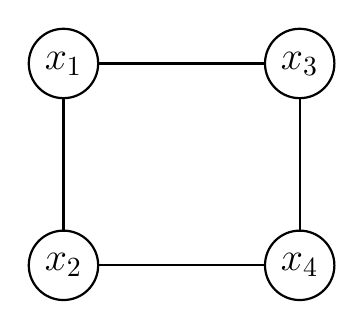
\begin{tikzpicture}[auto, node distance=3cm, every loop/.style={},
                    thick,main node/.style={circle,draw,font=\sffamily\Large\bfseries}]

  \node[main node] (1) {$x_1$};
  \node[main node] (2) [below =60] {$x_2$};
  \node[main node] (3) [right of=1] {$x_3$};
  \node[main node] (4) [right of=2] {$x_4$};

  \path[every node/.style={font=\sffamily\small}]
    (1) edge node [] {} (3)
    	edge node [] {} (2)
    (4) edge node [] {} (3)
    	edge node [] {}(2);
\end{tikzpicture}
\end{figure}
\begin{enumerate}
\examproblempart{To conduct MAP inference on this graph using exhaustive search, how many configurations must be checked?\\}
\bookletskip{0.2}

\framebox[14.7cm][l]{
	\begin{minipage}[b]{14.7cm}
	\inbooklet{Your answer: \MRFStudSolAA}
  
 	\solution{\MRFSolAA}
	\end{minipage}
 }
 
\examproblempart{Can MAP inference be run on this graph using a dynamic programming algorithm? Why or why not?\\}
\bookletskip{0.2}

\framebox[14.7cm][l]{
 	\begin{minipage}[b]{14.7cm}
 	\inbooklet{Your answer: \MRFStudSolAB}
  
 	\solution{\MRFSolAB}
 	\end{minipage}
 }
 \examproblempart{To run MAP inference on this graph using loopy belief propagation, how many messages must be computed?\\}
\bookletskip{0.2}

\framebox[14.7cm][l]{
 	\begin{minipage}[b]{14.7cm}
 	\inbooklet{Your answer: \MRFStudSolAC}
  
 	\solution{\MRFSolAC}
 	\end{minipage}
 }
 
\end{enumerate}

\examproblem{7}{ILP Inference formulation in Discrete Markov Random Fields}\\
\begin{enumerate}
\examproblempart{Suppose we have two variables $x_1\in\{0,1\}$ and $x_2\in\{0, 1\}$ and their local evidence functions $\theta_1(x_1)$ and $\theta_2(x_2)$ as well as a pairwise function $\theta_{1,2}(x_1,x_2)$. Using this setup, inference solves $\arg\max_{x_1,x_2} \theta_1(x_1) + \theta_2(x_2) + \theta_{1,2}(x_1,x_2)$. Using
\begin{align*}
\theta_1(x_1) &= \left\{\begin{array}{ll}1&\text{if~} x_1 = 0\\2&\text{otherwise}\end{array}\right. \quad
\theta_2(x_2) = \left\{\begin{array}{ll}1&\text{if~} x_2 = 0\\2&\text{otherwise}\end{array}\right. \\
\theta_{1,2}(x_1,x_2) &= \left\{\begin{array}{ll}-1& \text{otherwise}\\2&\text{if~}x_1 = 0 \text{~\&~} x_2 = 1\end{array}\right.
\end{align*}
what is the integer linear programming formulation of the inference task? Make the cost function and constraints explicit for the given problem, i.e., do not use a general formulation.

}
\bookletskip{0.2}   %in inches

% Solution box 
  \framebox[14.7cm][l]{
 \begin{minipage}[b]{14.7cm}
 \inbooklet{Your answer: \MRFStudSolBA}
  
 \solution{\MRFSolBA}
 \end{minipage}
 }

% Subproblem description
\examproblempart{What is the solution (value and argument) to the program in part (a). \\}
\bookletskip{0.2}   %in inches

% Solution box 
  \framebox[14.7cm][l]{
 \begin{minipage}[b]{14.7cm}
 \inbooklet{Your answer: \MRFStudSolBB}
  
 \solution{\MRFSolBB}
 \end{minipage}
 }

% Subproblem description 
 \examproblempart{Why do we typically not use the integer linear program for reasonably sized MRFs?
 }
 \bookletskip{0.2}   %in inches


% Solution box 
  \framebox[14.7cm][l]{
 \begin{minipage}[b]{14.7cm}
 \inbooklet{Your answer:  \MRFStudSolBC}
 
\solution{\MRFSolBC}
 \end{minipage}
 }
\end{enumerate}

\bookletpage
%%%%%%%%%%%% END OF PROBLEMS LIST
\end{enumerate}
\end{document}